\documentclass[twoside]{book}

% Packages required by doxygen
\usepackage{fixltx2e}
\usepackage{calc}
\usepackage{doxygen}
\usepackage[export]{adjustbox} % also loads graphicx
\usepackage{graphicx}
\usepackage[utf8]{inputenc}
\usepackage{makeidx}
\usepackage{multicol}
\usepackage{multirow}
\PassOptionsToPackage{warn}{textcomp}
\usepackage{textcomp}
\usepackage[nointegrals]{wasysym}
\usepackage[table]{xcolor}

% Font selection
\usepackage[T1]{fontenc}
\usepackage[scaled=.90]{helvet}
\usepackage{courier}
\usepackage{amssymb}
\usepackage{sectsty}
\renewcommand{\familydefault}{\sfdefault}
\allsectionsfont{%
  \fontseries{bc}\selectfont%
  \color{darkgray}%
}
\renewcommand{\DoxyLabelFont}{%
  \fontseries{bc}\selectfont%
  \color{darkgray}%
}
\newcommand{\+}{\discretionary{\mbox{\scriptsize$\hookleftarrow$}}{}{}}

% Page & text layout
\usepackage{geometry}
\geometry{%
  a4paper,%
  top=2.5cm,%
  bottom=2.5cm,%
  left=2.5cm,%
  right=2.5cm%
}
\tolerance=750
\hfuzz=15pt
\hbadness=750
\setlength{\emergencystretch}{15pt}
\setlength{\parindent}{0cm}
\setlength{\parskip}{3ex plus 2ex minus 2ex}
\makeatletter
\renewcommand{\paragraph}{%
  \@startsection{paragraph}{4}{0ex}{-1.0ex}{1.0ex}{%
    \normalfont\normalsize\bfseries\SS@parafont%
  }%
}
\renewcommand{\subparagraph}{%
  \@startsection{subparagraph}{5}{0ex}{-1.0ex}{1.0ex}{%
    \normalfont\normalsize\bfseries\SS@subparafont%
  }%
}
\makeatother

% Headers & footers
\usepackage{fancyhdr}
\pagestyle{fancyplain}
\fancyhead[LE]{\fancyplain{}{\bfseries\thepage}}
\fancyhead[CE]{\fancyplain{}{}}
\fancyhead[RE]{\fancyplain{}{\bfseries\leftmark}}
\fancyhead[LO]{\fancyplain{}{\bfseries\rightmark}}
\fancyhead[CO]{\fancyplain{}{}}
\fancyhead[RO]{\fancyplain{}{\bfseries\thepage}}
\fancyfoot[LE]{\fancyplain{}{}}
\fancyfoot[CE]{\fancyplain{}{}}
\fancyfoot[RE]{\fancyplain{}{\bfseries\scriptsize Generated by Doxygen }}
\fancyfoot[LO]{\fancyplain{}{\bfseries\scriptsize Generated by Doxygen }}
\fancyfoot[CO]{\fancyplain{}{}}
\fancyfoot[RO]{\fancyplain{}{}}
\renewcommand{\footrulewidth}{0.4pt}
\renewcommand{\chaptermark}[1]{%
  \markboth{#1}{}%
}
\renewcommand{\sectionmark}[1]{%
  \markright{\thesection\ #1}%
}

% Indices & bibliography
\usepackage{natbib}
\usepackage[titles]{tocloft}
\setcounter{tocdepth}{3}
\setcounter{secnumdepth}{5}
\makeindex

% Hyperlinks (required, but should be loaded last)
\usepackage{ifpdf}
\ifpdf
  \usepackage[pdftex,pagebackref=true]{hyperref}
\else
  \usepackage[ps2pdf,pagebackref=true]{hyperref}
\fi
\hypersetup{%
  colorlinks=true,%
  linkcolor=blue,%
  citecolor=blue,%
  unicode%
}

% Custom commands
\newcommand{\clearemptydoublepage}{%
  \newpage{\pagestyle{empty}\cleardoublepage}%
}

\usepackage{caption}
\captionsetup{labelsep=space,justification=centering,font={bf},singlelinecheck=off,skip=4pt,position=top}

%===== C O N T E N T S =====

\begin{document}

% Titlepage & ToC
\hypersetup{pageanchor=false,
             bookmarksnumbered=true,
             pdfencoding=unicode
            }
\pagenumbering{roman}
\begin{titlepage}
\vspace*{7cm}
\begin{center}%
{\Large Indexer }\\
\vspace*{1cm}
{\large Generated by Doxygen 1.8.11}\\
\end{center}
\end{titlepage}
\clearemptydoublepage
\tableofcontents
\clearemptydoublepage
\pagenumbering{arabic}
\hypersetup{pageanchor=true}

%--- Begin generated contents ---
\chapter{Hierarchical Index}
\section{Class Hierarchy}
This inheritance list is sorted roughly, but not completely, alphabetically\+:\begin{DoxyCompactList}
\item \contentsline{section}{H\+T\+M\+L\+Document}{\pageref{classHTMLDocument}}{}
\item \contentsline{section}{H\+T\+M\+L\+Document\+Parser}{\pageref{classHTMLDocumentParser}}{}
\item \contentsline{section}{I\+Stemmer}{\pageref{classIStemmer}}{}
\begin{DoxyCompactList}
\item \contentsline{section}{Stemmer}{\pageref{classStemmer}}{}
\end{DoxyCompactList}
\item \contentsline{section}{Worker}{\pageref{classWorker}}{}
\end{DoxyCompactList}

\chapter{Class Index}
\section{Class List}
Here are the classes, structs, unions and interfaces with brief descriptions\+:\begin{DoxyCompactList}
\item\contentsline{section}{\hyperlink{classHTMLDocument}{H\+T\+M\+L\+Document} }{\pageref{classHTMLDocument}}{}
\item\contentsline{section}{\hyperlink{classHTMLDocumentParser}{H\+T\+M\+L\+Document\+Parser} }{\pageref{classHTMLDocumentParser}}{}
\item\contentsline{section}{\hyperlink{classIStemmer}{I\+Stemmer} }{\pageref{classIStemmer}}{}
\item\contentsline{section}{\hyperlink{classStemmer}{Stemmer} }{\pageref{classStemmer}}{}
\item\contentsline{section}{\hyperlink{classWorker}{Worker} }{\pageref{classWorker}}{}
\end{DoxyCompactList}

\chapter{Class Documentation}
\hypertarget{classHTMLDocument}{}\section{H\+T\+M\+L\+Document Class Reference}
\label{classHTMLDocument}\index{H\+T\+M\+L\+Document@{H\+T\+M\+L\+Document}}


{\ttfamily \#include $<$H\+T\+M\+L\+Document.\+h$>$}

\subsection*{Public Member Functions}
\begin{DoxyCompactItemize}
\item 
{\bfseries H\+T\+M\+L\+Document} (const std\+::string \&html)\hypertarget{classHTMLDocument_a98e4e50ff2b4fe3b13cea21e3094e80d}{}\label{classHTMLDocument_a98e4e50ff2b4fe3b13cea21e3094e80d}

\item 
{\bfseries H\+T\+M\+L\+Document} (std\+::string \&\&html)\hypertarget{classHTMLDocument_acc0354fc26aac69b2fd1a04706c1e25f}{}\label{classHTMLDocument_acc0354fc26aac69b2fd1a04706c1e25f}

\item 
void \hyperlink{classHTMLDocument_a20196a45d63965ad7c9860079adbf779}{parse} ()
\begin{DoxyCompactList}\small\item\em parse html code. \end{DoxyCompactList}\item 
unsigned long {\bfseries get\+Id} () const \hypertarget{classHTMLDocument_a28fa57f3d55f2dd1a4f7cbb3fd544200}{}\label{classHTMLDocument_a28fa57f3d55f2dd1a4f7cbb3fd544200}

\item 
void {\bfseries set\+Id} (unsigned long id)\hypertarget{classHTMLDocument_a445aad9a305d71d496e52c935fab720e}{}\label{classHTMLDocument_a445aad9a305d71d496e52c935fab720e}

\item 
const std\+::string \& {\bfseries get\+Html} () const \hypertarget{classHTMLDocument_acff4c5828290b6997d9c29f69bdc5915}{}\label{classHTMLDocument_acff4c5828290b6997d9c29f69bdc5915}

\item 
bool \hyperlink{classHTMLDocument_a26d4250db9a7b0dfdd103c4ad4fb4b99}{set\+Html} (const std\+::string \&html)
\begin{DoxyCompactList}\small\item\em Set html code. \end{DoxyCompactList}\item 
bool {\bfseries set\+Html} (std\+::string \&\&html)\hypertarget{classHTMLDocument_aceba92aefa58d39ba06466199580e693}{}\label{classHTMLDocument_aceba92aefa58d39ba06466199580e693}

\item 
const std\+::string \& {\bfseries get\+Text} () const \hypertarget{classHTMLDocument_a575b82acaa32219ef65b8ed1be818bab}{}\label{classHTMLDocument_a575b82acaa32219ef65b8ed1be818bab}

\item 
void {\bfseries set\+Text} (const std\+::string \&text)\hypertarget{classHTMLDocument_a9f21e2c958db4e300fdf5ae314981df3}{}\label{classHTMLDocument_a9f21e2c958db4e300fdf5ae314981df3}

\item 
const std\+::vector$<$ std\+::string $>$ \& {\bfseries get\+Tokens} () const \hypertarget{classHTMLDocument_a34cc34993ff60ebfe0b033ed11a8341a}{}\label{classHTMLDocument_a34cc34993ff60ebfe0b033ed11a8341a}

\item 
void {\bfseries set\+Tokens} (const std\+::vector$<$ std\+::string $>$ \&tokens)\hypertarget{classHTMLDocument_afd3e0702fb251d9340c7ab3780f637cc}{}\label{classHTMLDocument_afd3e0702fb251d9340c7ab3780f637cc}

\item 
bool {\bfseries is\+Valid} () const \hypertarget{classHTMLDocument_a995ec1bb3ae82cd90b227e3f842f52fe}{}\label{classHTMLDocument_a995ec1bb3ae82cd90b227e3f842f52fe}

\end{DoxyCompactItemize}


\subsection{Detailed Description}
Stores all the document\textquotesingle{}s data 

\subsection{Member Function Documentation}
\index{H\+T\+M\+L\+Document@{H\+T\+M\+L\+Document}!parse@{parse}}
\index{parse@{parse}!H\+T\+M\+L\+Document@{H\+T\+M\+L\+Document}}
\subsubsection[{\texorpdfstring{parse()}{parse()}}]{\setlength{\rightskip}{0pt plus 5cm}void H\+T\+M\+L\+Document\+::parse (
\begin{DoxyParamCaption}
{}
\end{DoxyParamCaption}
)}\hypertarget{classHTMLDocument_a20196a45d63965ad7c9860079adbf779}{}\label{classHTMLDocument_a20196a45d63965ad7c9860079adbf779}


parse html code. 

Checks if the html code is valid. Uses \hyperlink{classHTMLDocumentParser}{H\+T\+M\+L\+Document\+Parser}. \index{H\+T\+M\+L\+Document@{H\+T\+M\+L\+Document}!set\+Html@{set\+Html}}
\index{set\+Html@{set\+Html}!H\+T\+M\+L\+Document@{H\+T\+M\+L\+Document}}
\subsubsection[{\texorpdfstring{set\+Html(const std\+::string \&html)}{setHtml(const std::string &html)}}]{\setlength{\rightskip}{0pt plus 5cm}bool H\+T\+M\+L\+Document\+::set\+Html (
\begin{DoxyParamCaption}
\item[{const std\+::string \&}]{html}
\end{DoxyParamCaption}
)}\hypertarget{classHTMLDocument_a26d4250db9a7b0dfdd103c4ad4fb4b99}{}\label{classHTMLDocument_a26d4250db9a7b0dfdd103c4ad4fb4b99}


Set html code. 


\begin{DoxyParams}{Parameters}
{\em html} & \\
\hline
\end{DoxyParams}
\begin{DoxyReturn}{Returns}
whether the html code is valid or not 
\end{DoxyReturn}


The documentation for this class was generated from the following files\+:\begin{DoxyCompactItemize}
\item 
src/index/H\+T\+M\+L\+Document.\+h\item 
src/index/H\+T\+M\+L\+Document.\+cpp\end{DoxyCompactItemize}

\hypertarget{classHTMLDocumentParser}{}\section{H\+T\+M\+L\+Document\+Parser Class Reference}
\label{classHTMLDocumentParser}\index{H\+T\+M\+L\+Document\+Parser@{H\+T\+M\+L\+Document\+Parser}}


{\ttfamily \#include $<$H\+T\+M\+L\+Document\+Parser.\+h$>$}

\subsection*{Public Member Functions}
\begin{DoxyCompactItemize}
\item 
bool {\bfseries is\+H\+T\+M\+L\+Valid} (std\+::string \&html)\hypertarget{classHTMLDocumentParser_a30e99ba7e6164ab947b8521e8a560b66}{}\label{classHTMLDocumentParser_a30e99ba7e6164ab947b8521e8a560b66}

\item 
std\+::string \hyperlink{classHTMLDocumentParser_af6e652d8ebeaba42076efb746745db15}{extract\+Text} (const std\+::string \&html)
\begin{DoxyCompactList}\small\item\em extract text of a page from html code \end{DoxyCompactList}\item 
std\+::vector$<$ std\+::string $>$ \hyperlink{classHTMLDocumentParser_af1dd1a2f93dcb83aacf61c4a4623511f}{extract\+Links} (const std\+::string \&html)
\begin{DoxyCompactList}\small\item\em extract links from a page \end{DoxyCompactList}\end{DoxyCompactItemize}


\subsection{Detailed Description}
Operations on html code 

\subsection{Member Function Documentation}
\index{H\+T\+M\+L\+Document\+Parser@{H\+T\+M\+L\+Document\+Parser}!extract\+Links@{extract\+Links}}
\index{extract\+Links@{extract\+Links}!H\+T\+M\+L\+Document\+Parser@{H\+T\+M\+L\+Document\+Parser}}
\subsubsection[{\texorpdfstring{extract\+Links(const std\+::string \&html)}{extractLinks(const std::string &html)}}]{\setlength{\rightskip}{0pt plus 5cm}vector$<$ string $>$ H\+T\+M\+L\+Document\+Parser\+::extract\+Links (
\begin{DoxyParamCaption}
\item[{const std\+::string \&}]{html}
\end{DoxyParamCaption}
)}\hypertarget{classHTMLDocumentParser_af1dd1a2f93dcb83aacf61c4a4623511f}{}\label{classHTMLDocumentParser_af1dd1a2f93dcb83aacf61c4a4623511f}


extract links from a page 


\begin{DoxyParams}{Parameters}
{\em html} & source code of the page \\
\hline
\end{DoxyParams}
\begin{DoxyReturn}{Returns}
array of links from the page 
\end{DoxyReturn}
\index{H\+T\+M\+L\+Document\+Parser@{H\+T\+M\+L\+Document\+Parser}!extract\+Text@{extract\+Text}}
\index{extract\+Text@{extract\+Text}!H\+T\+M\+L\+Document\+Parser@{H\+T\+M\+L\+Document\+Parser}}
\subsubsection[{\texorpdfstring{extract\+Text(const std\+::string \&html)}{extractText(const std::string &html)}}]{\setlength{\rightskip}{0pt plus 5cm}string H\+T\+M\+L\+Document\+Parser\+::extract\+Text (
\begin{DoxyParamCaption}
\item[{const std\+::string \&}]{html}
\end{DoxyParamCaption}
)}\hypertarget{classHTMLDocumentParser_af6e652d8ebeaba42076efb746745db15}{}\label{classHTMLDocumentParser_af6e652d8ebeaba42076efb746745db15}


extract text of a page from html code 


\begin{DoxyParams}{Parameters}
{\em html} & source code of the page \\
\hline
\end{DoxyParams}
\begin{DoxyReturn}{Returns}
plain text from the page
\end{DoxyReturn}
Wrapper around gumbo library. Uses internal dump\+Text method recursively to parse html code. 

The documentation for this class was generated from the following files\+:\begin{DoxyCompactItemize}
\item 
src/parser/H\+T\+M\+L\+Document\+Parser.\+h\item 
src/parser/H\+T\+M\+L\+Document\+Parser.\+cpp\end{DoxyCompactItemize}

\hypertarget{classIStemmer}{}\section{I\+Stemmer Class Reference}
\label{classIStemmer}\index{I\+Stemmer@{I\+Stemmer}}
Inheritance diagram for I\+Stemmer\+:\begin{figure}[H]
\begin{center}
\leavevmode
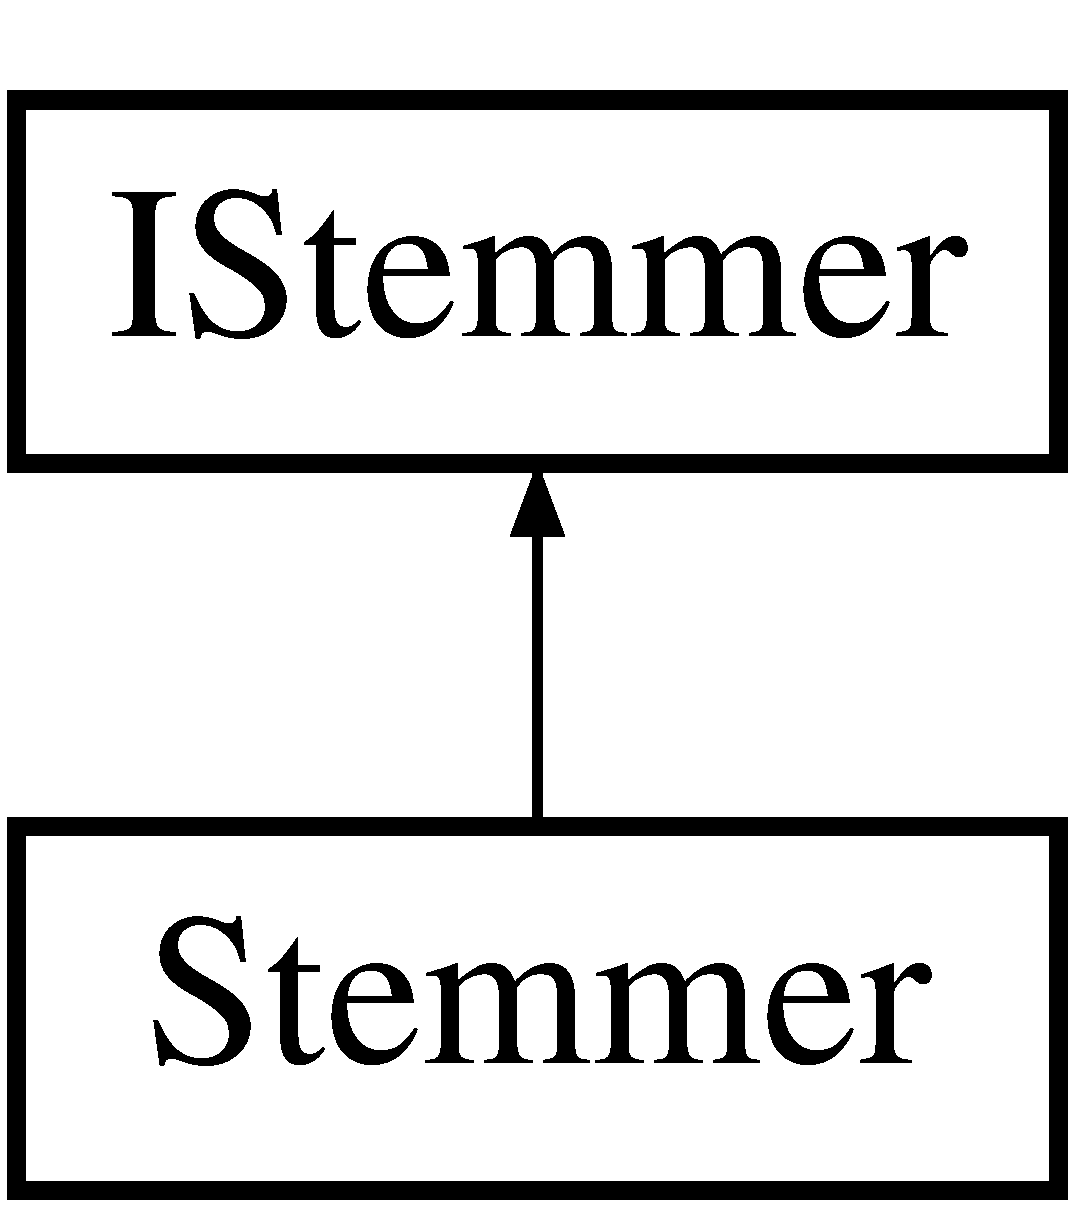
\includegraphics[height=2.000000cm]{classIStemmer}
\end{center}
\end{figure}


The documentation for this class was generated from the following file\+:\begin{DoxyCompactItemize}
\item 
src/index/I\+Stemmer.\+h\end{DoxyCompactItemize}

\hypertarget{classStemmer}{}\section{Stemmer Class Reference}
\label{classStemmer}\index{Stemmer@{Stemmer}}


{\ttfamily \#include $<$Stemmer.\+h$>$}

Inheritance diagram for Stemmer\+:\begin{figure}[H]
\begin{center}
\leavevmode
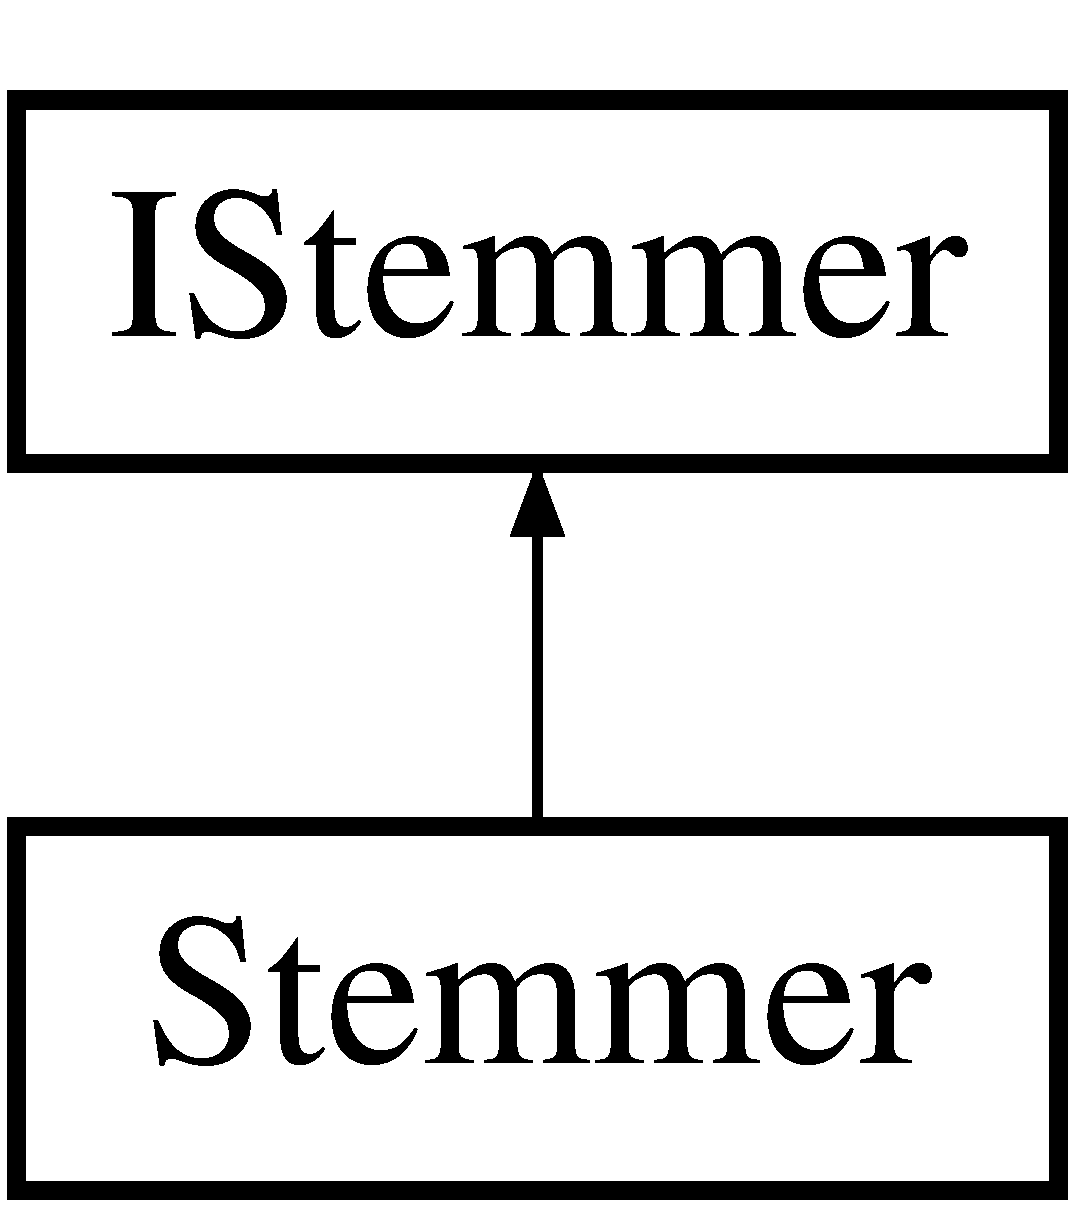
\includegraphics[height=2.000000cm]{classStemmer}
\end{center}
\end{figure}
\subsection*{Public Member Functions}
\begin{DoxyCompactItemize}
\item 
std\+::vector$<$ std\+::string $>$ \& {\bfseries stem} (std\+::vector$<$ std\+::string $>$ \&) const override\hypertarget{classStemmer_ae058747c8ba219324631ddd0e7258d9e}{}\label{classStemmer_ae058747c8ba219324631ddd0e7258d9e}

\item 
unsigned int {\bfseries measure} (std\+::string word) const \hypertarget{classStemmer_a221809125f65c5c3154fa4c482e39f9b}{}\label{classStemmer_a221809125f65c5c3154fa4c482e39f9b}

\item 
std\+::string \& {\bfseries step1} (std\+::string \&)\hypertarget{classStemmer_a8a77a75e099f66edcafbbdb6b6b824c4}{}\label{classStemmer_a8a77a75e099f66edcafbbdb6b6b824c4}

\item 
std\+::string \& {\bfseries step1c} (std\+::string \&)\hypertarget{classStemmer_a8b84eb574cf401df2530aab31b234b8b}{}\label{classStemmer_a8b84eb574cf401df2530aab31b234b8b}

\item 
std\+::string \& {\bfseries step2} (std\+::string \&)\hypertarget{classStemmer_ad68bf0a9c083172fc928598171eee393}{}\label{classStemmer_ad68bf0a9c083172fc928598171eee393}

\item 
std\+::string \& {\bfseries step3} (std\+::string \&)\hypertarget{classStemmer_a4dc45e7fd247a8490d2dbf7e31bc75f2}{}\label{classStemmer_a4dc45e7fd247a8490d2dbf7e31bc75f2}

\item 
std\+::string \& {\bfseries step4} (std\+::string \&)\hypertarget{classStemmer_a8e8eaaac711dd39e1b3caccd8bcdfd7b}{}\label{classStemmer_a8e8eaaac711dd39e1b3caccd8bcdfd7b}

\item 
std\+::string \& {\bfseries step5} (std\+::string \&)\hypertarget{classStemmer_a251f8e0b66f18f511d00e77963e0664f}{}\label{classStemmer_a251f8e0b66f18f511d00e77963e0664f}

\item 
std\+::string \& {\bfseries step6} (std\+::string \&)\hypertarget{classStemmer_a4b3dd324562043bc7654e46fcef8ae47}{}\label{classStemmer_a4b3dd324562043bc7654e46fcef8ae47}

\end{DoxyCompactItemize}


\subsection{Detailed Description}
Porter`s stemming algorithm 

The documentation for this class was generated from the following files\+:\begin{DoxyCompactItemize}
\item 
src/index/Stemmer.\+h\item 
src/index/Stemmer.\+cpp\end{DoxyCompactItemize}

\hypertarget{classWorker}{}\section{Worker Class Reference}
\label{classWorker}\index{Worker@{Worker}}


{\ttfamily \#include $<$Worker.\+h$>$}

\subsection*{Public Member Functions}
\begin{DoxyCompactItemize}
\item 
{\bfseries Worker} (\hyperlink{classWorker}{Worker} \&)=delete\hypertarget{classWorker_a0fb59883eb34da625420e40141dd29b2}{}\label{classWorker_a0fb59883eb34da625420e40141dd29b2}

\item 
\hyperlink{classWorker}{Worker} \& {\bfseries operator=} (const \hyperlink{classWorker}{Worker} \&)=delete\hypertarget{classWorker_aca397cd5d556133de9f7868127a920f5}{}\label{classWorker_aca397cd5d556133de9f7868127a920f5}

\item 
{\bfseries Worker} (\hyperlink{classWorker}{Worker} \&\&)=default\hypertarget{classWorker_a0c825b0d290c3c131f7a21758baefd66}{}\label{classWorker_a0c825b0d290c3c131f7a21758baefd66}

\item 
\hyperlink{classWorker}{Worker} \& {\bfseries operator=} (\hyperlink{classWorker}{Worker} \&\&)=default\hypertarget{classWorker_a3840f121930b58702dcba26b5e0dd83f}{}\label{classWorker_a3840f121930b58702dcba26b5e0dd83f}

\item 
void \hyperlink{classWorker_a251fee1d1e2715c5606939b5080c8488}{start} (\hyperlink{classHTMLDocument}{H\+T\+M\+L\+Document} \&) const 
\begin{DoxyCompactList}\small\item\em start indexing a web page \end{DoxyCompactList}\item 
std\+::vector$<$ std\+::string $>$ \hyperlink{classWorker_a25d6fba1b641c77bb0565df8b1de12ad}{tokenize} (std\+::string \&) const 
\begin{DoxyCompactList}\small\item\em split text into a list of tokens \end{DoxyCompactList}\item 
std\+::vector$<$ std\+::string $>$ \& \hyperlink{classWorker_addf90002a4063b5a8b23de39d151d19a}{stem} (std\+::vector$<$ std\+::string $>$ \&) const 
\end{DoxyCompactItemize}


\subsection{Detailed Description}
Manages indexing loop 

\subsection{Member Function Documentation}
\index{Worker@{Worker}!start@{start}}
\index{start@{start}!Worker@{Worker}}
\subsubsection[{\texorpdfstring{start(\+H\+T\+M\+L\+Document \&) const }{start(HTMLDocument &) const }}]{\setlength{\rightskip}{0pt plus 5cm}void Worker\+::start (
\begin{DoxyParamCaption}
\item[{{\bf H\+T\+M\+L\+Document} \&}]{page}
\end{DoxyParamCaption}
) const}\hypertarget{classWorker_a251fee1d1e2715c5606939b5080c8488}{}\label{classWorker_a251fee1d1e2715c5606939b5080c8488}


start indexing a web page 

Starts indexing loop\+: read a html file from the source dir, parse it, tokenize, stemm and add to index. \index{Worker@{Worker}!stem@{stem}}
\index{stem@{stem}!Worker@{Worker}}
\subsubsection[{\texorpdfstring{stem(std\+::vector$<$ std\+::string $>$ \&) const }{stem(std::vector< std::string > &) const }}]{\setlength{\rightskip}{0pt plus 5cm}vector$<$ string $>$ \& Worker\+::stem (
\begin{DoxyParamCaption}
\item[{std\+::vector$<$ std\+::string $>$ \&}]{tokens}
\end{DoxyParamCaption}
) const}\hypertarget{classWorker_addf90002a4063b5a8b23de39d151d19a}{}\label{classWorker_addf90002a4063b5a8b23de39d151d19a}
Tokens stemming. 
\begin{DoxyParams}{Parameters}
{\em list} & of tokens \\
\hline
\end{DoxyParams}
\begin{DoxyReturn}{Returns}
list of stemmed tokens
\end{DoxyReturn}
Porter`s algorithm \index{Worker@{Worker}!tokenize@{tokenize}}
\index{tokenize@{tokenize}!Worker@{Worker}}
\subsubsection[{\texorpdfstring{tokenize(std\+::string \&) const }{tokenize(std::string &) const }}]{\setlength{\rightskip}{0pt plus 5cm}vector$<$ string $>$ Worker\+::tokenize (
\begin{DoxyParamCaption}
\item[{std\+::string \&}]{text}
\end{DoxyParamCaption}
) const}\hypertarget{classWorker_a25d6fba1b641c77bb0565df8b1de12ad}{}\label{classWorker_a25d6fba1b641c77bb0565df8b1de12ad}


split text into a list of tokens 


\begin{DoxyParams}{Parameters}
{\em text} & to tokenize \\
\hline
\end{DoxyParams}
\begin{DoxyReturn}{Returns}
a vector of tokens 
\end{DoxyReturn}


The documentation for this class was generated from the following files\+:\begin{DoxyCompactItemize}
\item 
src/index/Worker.\+h\item 
src/index/Worker.\+cpp\end{DoxyCompactItemize}

%--- End generated contents ---

% Index
\backmatter
\newpage
\phantomsection
\clearemptydoublepage
\addcontentsline{toc}{chapter}{Index}
\printindex

\end{document}
